\documentclass[11pt,a4paper]{article}

% Packages
\usepackage{graphicx} % For including images
\usepackage{hyperref} % For including hyperlinks
\usepackage{cite} % For citations
\usepackage{bm} % For bold math symbols
\usepackage{geometry} % For setting page margins
\usepackage{setspace} % For setting line spacing
\usepackage[vlined,ruled,linesnumbered]{algorithm2e} % For writing algorithms
\usepackage{indentfirst} % For indenting the first paragraph of a section

\geometry{
    left=1.2in,
    right=1.2in,
    top=1in,
    bottom=1in
} 




% Title
\title{Technical Report about Operating System Supports for Database}
\author{Yiheng Bing  522031910191}
\date{\today}

\begin{document}

\maketitle

\fontsize{10pt}{12pt}

\setstretch{1.2}

\begin{abstract}
As the amount of data grows, the demand for database systems is increasing. 
Database systems are widely used in various fields, such as e-commerce, social networks, and scientific research.
However, the traditional operating systems can not fit the requirements of database systems well.
To meet the requirements of different applications, database systems need to be optimized for performance, reliability, and scalability. 
Database systems need to be optimized for performance, reliability, and scalability.
Operating system support is essential for database systems to achieve high performance, reliability, and scalability.
In this report, we will discuss the operating system supports for database systems and how they can be optimized to improve performance and scalability.
We will focus on memory management, process scheduling, and file system management, and discuss how these aspects can be optimized to support database systems.
\end{abstract}

\tableofcontents
\newpage


\section{Introduction}
Database is an organized collection of data, typically stored and accessed electronically from a computer system. 
Small databases can be stored on a single computer, while large databases are often spread out over networked computers, making the data accessible to multiple users and applications.
More than 40 years ago, Stonebraker published a paper on the topic of operating system support for database management systems (DBMS).
In this paper, he argued that the operating system should provide higher-level support for DBMS to improve performance and reliability.
He said that database management systems (DBMS) provide higher level user support than conventional operating systems, 
and the DBMS designer must work in the context of the OS he/she is faced with. 
Different operating systems are designed for different use.  \cite{10.1145/358699.358703}
In this report, I will discuss the development of database systems in this years and the optimization of operating system support for database systems.

\begin{figure}[h!]
    \centering
    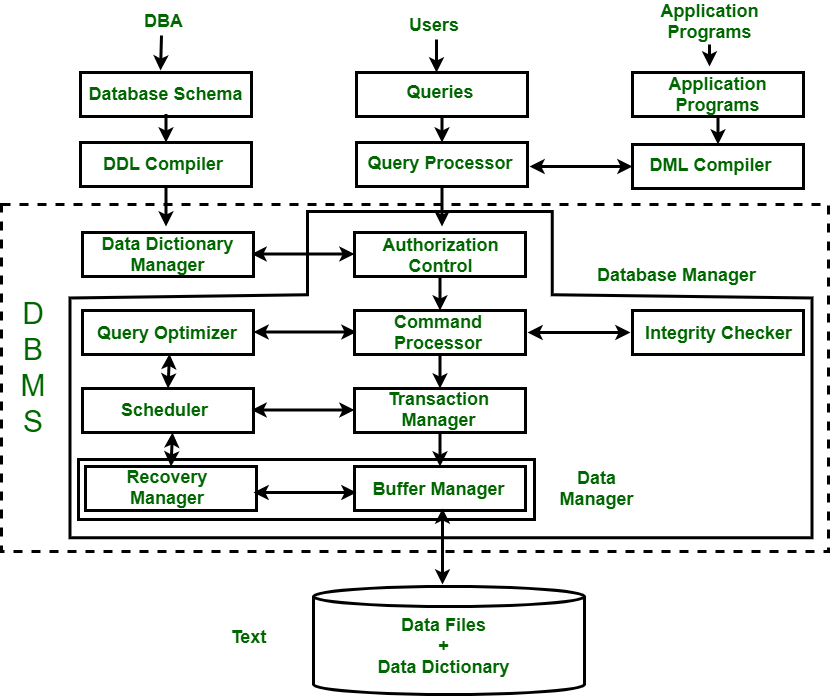
\includegraphics[width=0.6\textwidth]{DBMS.png}
    \caption{Structure of Database Management System}
\end{figure}
\section{Memory Management}

\subsection{Memory Management in Operating System}

In traditional operating systems, memory management is a fundamental aspect. 
The operating system is responsible for managing the memory resources of the computer system, including allocating and deallocating memory, protecting memory, and providing virtual memory support.
Most operating systems use a hirarchical memory management system, which divides the memory into different levels of memory, such as physical memory, virtual memory, and cache memory.
And the cache memory is used to store frequently accessed data to improve performance.
Also, operating systems provide virtual memory support to allow processes to use more memory than the physical memory available on the system. 

\subsection{Requirements of Memory Management for Database Systems}
\begin{enumerate}
    \item \textbf{Large capacity memory support}
    
    Databases usually need to handle large amounts of data, so the memory requirements are also high. 
    The operating system should support large-capacity physical memory so that the database can cache large amounts of data and reduce the dependency on disk I/O, thus improving access efficiency.
    
    \item \textbf{Efficient memory allocation and reclamation mechanism}
    
    Database systems need to allocate and free memory frequently, so database systems needs fast and efficient memory allocation and reclamation mechanisms to reduce memory fragmentation and improve memory usage efficiency.
    
    \item \textbf{Virtual memory and memory mapping}
    
    The operating system uses the virtual memory mechanism to enable the database system to use a larger address space than the actual physical memory. 
    The memory-mapped file feature allows the database to map disk files directly in the process address space, which helps to improve the efficiency of disk I/O operations.
    
\end{enumerate}

\subsection{Optimization of Memory Management for Database Systems}

To optimize memory management for database systems, the operating system can use techniques such as huge pages, memory pooling, and virtual memory.
\begin{enumerate}
    \item \textbf{Huge pages}
    
        In order to improve the efficiency of large-scale data processing when dealing with a huge amount of data, the operating system should support the HugePages function, 
    which can reduce the size of the page table and reduce the probability of missing TLB (Translation Lookaside Buffer), thereby improving performance.

    \item \textbf{Memory pooling}
    
        Memory pooling is a technique that allows the database system to allocate and free memory in a more efficient way.
    By pre-allocating a pool of memory blocks of fixed size, the database system can reduce the overhead of memory allocation and deallocation,
    and improve the performance of memory management.
    
    \item \textbf{Virtual memory}
    
        Virtual memory is a key feature of modern operating systems that allows processes to use more memory than the physical memory available on the system.
    By using virtual memory, the database system can reduce the dependency on disk I/O and improve the performance of memory-intensive operations.
    Mapping files into virtual memory may be an elegant and efficient approach, but that additional function is needed to support the recovery requirements of database systems and transaction processing.
    Shadow paging scheme and WAL(Write Ahead Log) are two approaches that offer an indication of the work that may be needed. 

    \item \textbf{Shadow paging scheme}
    
        Shadow paging scheme is a technique that allows the database system to maintain a shadow copy of the database in memory and update the shadow copy instead of the original database.
    This technique can improve the performance of database, accelerate memory recovery and reduce the overhead of logging and checkpointing, and interactions across RSS components are relatively simple 
    because they don't have to log individual changes to their pages during normal forward processings.\cite{10.1145/850726.850729} 
    Also, for the shadow page itself a kind of log, so that the recovery process can be simplified and the information to be writed down to log is greatly reduced, too.

    \begin{figure}[h!]
        \centering
        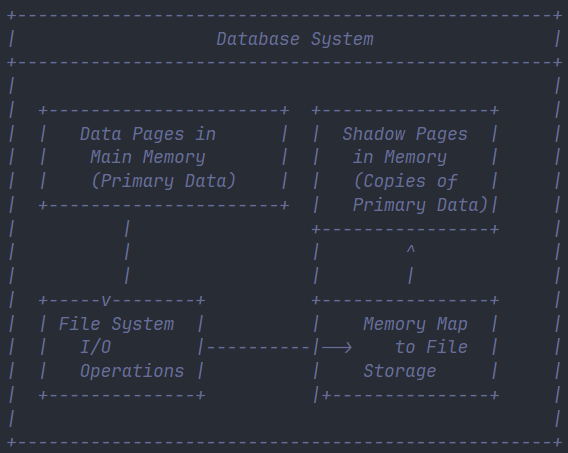
\includegraphics[width=0.6\textwidth]{shadowpage.png}
        \caption{Shadow Paging Scheme}
    \end{figure}


    \item \textbf{Write Ahead Log}
    
        Write ahead log is a technique that requires the database system to write the log records to disk before writing the corresponding data to disk.
    In a WAL scheme, each page has only one home location, and all I/0 operations are directed to that location. 
    There is no notion of moving the page to any other location, or forming a shadow copy of its old or new contents. 
    However, before the data page is written to disk, the log buffer must first be written to disk if it contains one or more log entries for that data page.\cite{10.1145/850726.850729}

\end{enumerate}
\section{Process Scheduling}

Process scheduling is another important aspect of operating system support for database systems.
Database systems need to manage multiple concurrent transactions and queries efficiently.
The operating system provides services such as process scheduling, synchronization, and inter-process communication to support database systems.
To optimize process scheduling for database systems, the operating system can use techniques or policies such as data-centric architecture, least-loaded scheduler, self-adaptive via modern ml and so on.
These techniques can help improve the scalability and performance of database systems by efficiently utilizing the available resources.

\subsection{Data-Centric Architecture}

Data-Centric Architecture is a new approach to database system design that focuses on optimizing data access and processing.
In a data-centric architecture, the database system is designed to be data-aware and data-driven, which means that the system is optimized for data access and processing.
The operating system can support data-centric architecture by providing services such as data caching, data partitioning, and data replication.
These services can help improve the performance and scalability of database systems by reducing the latency of data access and processing.

In this architecture, DBMS will get better scheduling. 
There will be task and resource tables in the DBMS capturing what tasks runs on cores, chips, nodes, and datacenters and what resources are available. 
Scheduling thousands of parallel tasks in such environments as Map-Reduce and Spark is 
mainly an exercise in finding available resources and stragglers, because running time is the time of the slowest parallel task. 
Finding outliers in a large task table is merely a decision support query that can be coded in SQL. 
Again, we believe that the additional functionality can be provided at a net savings in code.\cite{10.1007/978-3-030-71055-2_1}

\begin{figure}[h!]
    \centering
    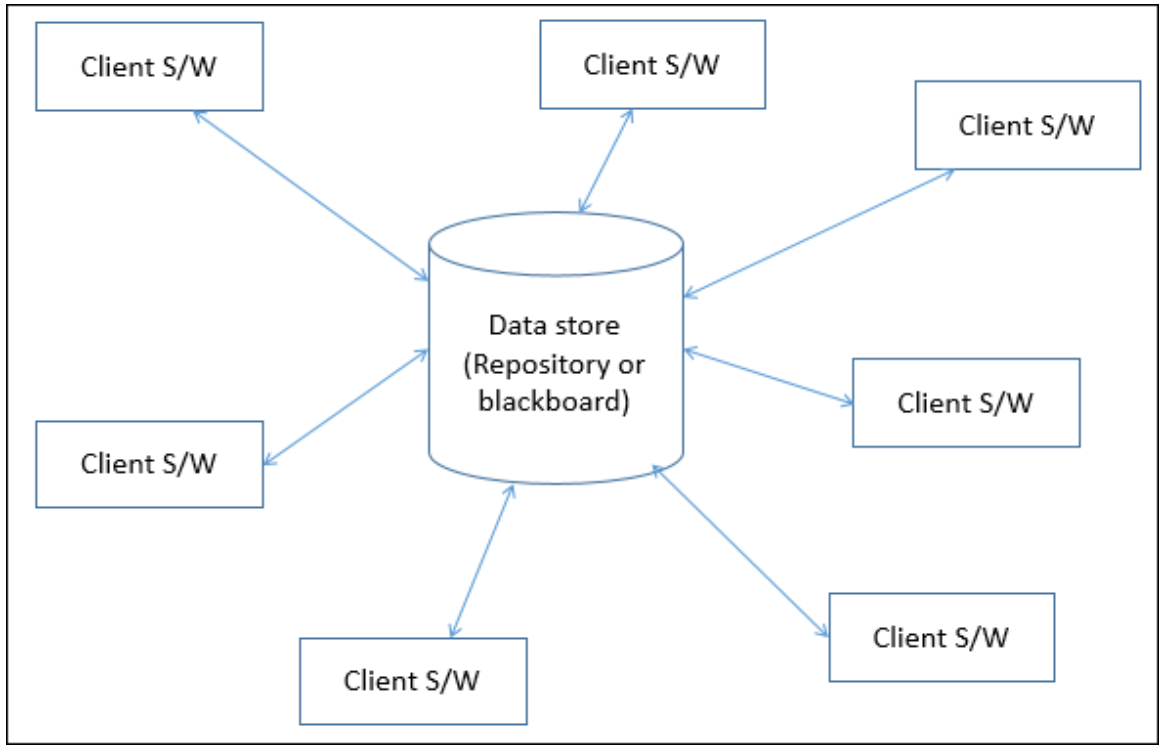
\includegraphics[width=0.6\textwidth]{datacenarch.png}
    \caption{Data-Centric Architecture}
\end{figure}

\subsection{Least-Loaded Scheduler}

Least-Loaded Scheduler is a scheduling policy that assigns tasks to the least-loaded processor or resource.
This policy can help balance the load across multiple processors or resources and improve the performance of database systems.
The operating system can support the least-loaded scheduler by providing services such as load balancing, task migration, and resource allocation.
These services can help optimize the scheduling of tasks and improve the scalability of database systems.

The least-loaded scheduler ensures the best load balance possible, assuming fairly long running tasks. 
This scheduling strategy is commonly used in many existing systems.
Specifically, we schedule the next incoming task to the worker with the greatest unused capacity within a partition.\cite{10.14778/3485450.3485454}

In the following algorithms, we can see the difference between the simple FIFO scheduler and the least-loaded scheduler. We need only change a little part of the code in the algorithm, 
and we can easily find that the least-loaded scheduler is just slightly slower than the FIFO scheduler in Figure4.

\begin{minipage}[t]{0.9\textwidth}
    \begin{algorithm}[H]
        \KwIn{select $worker\_id, unused\_capacity$ from Worker where $unused\_capacity > 0$, $p\_key = P$, $limit = 1$;}
        
        \BlankLine
        \caption{Simple FIFO Scheduler}
        
        \uIf{$worker\_id$ is not NONE}{
            $WID = worker\_id[0]$\;
            $UC = unused\_capacity[0]$\;
            update Worker set $W$\;
                $(unused\_capacity = UC - 1$ \;
                where $worker\_id = WID$ and $p\_key = P)$\;
            insert into Task $T$ with $worker\_id = WID$ and $task\_id = TID$\;
        }
    \end{algorithm}
\end{minipage}

\begin{minipage}[t]{0.9\textwidth}
    \begin{algorithm}[H]
        \KwIn{select $worker\_id, unused\_capacity$ from Worker where $unused\_capacity > 0$, $p\_key = P$, $limit = 1$;}
        
        \BlankLine
        \caption{Least-Loaded Scheduler}
        order by $unused\_capacity$\;
        \uIf{$worker\_id$ is not NONE}{
            $WID = worker\_id[0]$\;
            $UC = unused\_capacity[0]$\;
            update Worker set $W$\;
                $(unused\_capacity = UC - 1$ \;
                where $worker\_id = WID$ and $p\_key = P)$\;
            
                
            insert into Task $T$ with $worker\_id = WID$ and $task\_id = TID$\;
        }
    \end{algorithm}
\end{minipage}


\begin{figure}[h!]
    \centering
    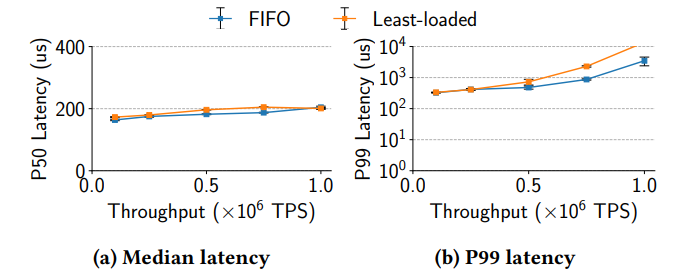
\includegraphics[width=0.8\textwidth]{latency.png}
    \caption{Comparison of Two Schedulers}
\end{figure}

\subsection{Self-adaptive via Modern ML}

Self-adaptive via Modern ML is a new approach that aims to automate and optimize the process of scheduling tasks based on the current workload and data characteristics.
In this approach, the operating system uses machine learning algorithms to learn the patterns of task execution and resource usage and adapt the scheduling policy accordingly.
This approach can help improve the performance and scalability of database systems by dynamically adjusting the scheduling policy based on the workload and system conditions.



Sometimes, the optimal scheduling policy may not be the most suitable for some workloads and data, we can use modern ml to help with predicting and self-adaptive. 
To address a wide range of use cases, the system developer often has to make algorithmic compromises. 
For instance, every operating system requires a scheduling algorithm, but the chosen scheduling algorithm might not be optimal under all workloads or hardware types. 
In order to provide the best performance, we envision that the system is able to automatically switch the algorithm used, based on the workload and data. 
This would apply to scheduling, memory management, etc.\cite{10.1007/978-3-030-71055-2_1}
And additionally, ml is good at such according tasks when with known workloads or relative data as inputs. 

The prosperity of machine learning (ML), especially deep learning, helps to resolve a large number of DBMS challenges.
ML techniques enable automatic, fine-grained, and more accurate characterization of the problem space and benefit a variety of tasks in DBMS.\cite{DBLP:journals/corr/abs-2105-02418}
It would also help DBMS to optimize the scheduling policy according to the conditions.

\begin{figure}[h!]
    \centering
    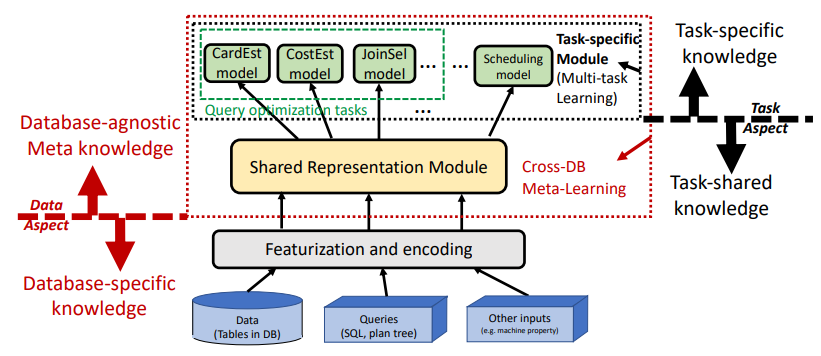
\includegraphics[width=0.8\textwidth]{mlpre.png}
    \caption{Self-adaptive via Modern ML}
\end{figure}

\section{File System Management}

File system management is also crucial for operating system support for database systems.
Database systems need to store and retrieve data efficiently from disk storage.
So the database file system(DBFS) has a higher standard than normal file systems.
The design of DBFS is simplified by the use of powerful database primitives such as transactions, fine-grained locking, and write-ahead logging.\cite{10.14778/2536360.2536361}
Usually, the architecture of DBFS would be organized as following Figure6.
To optimize file system management for database systems, the operating system can use techniques such as hybrid storage, query optimization and so on.
These techniques can help reduce the latency of disk I/O operations and improve the performance of database systems.

\begin{figure}[h!]
    \centering
    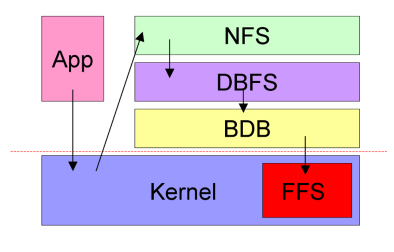
\includegraphics[width=0.6\textwidth]{dbfsarch.png}
    \caption{DBFS architecture}
\end{figure}

\subsection{Hybrid storage}

Hybrid storage is a technique that allows the database system to store data in  both flash-based solid state drives (SSDs) and traditional hard disk drives (HDDs), whose architecture is shown as following Figure7.
However, adding SSDs to a storage system not only raises the question of how to manage the SSDs, but also raises the question of whether current buffer pool algorithms will still work effectively.
As database systems have great demand of data storage and high-level concurrent data access, the hybrid storage is a good choice.
These services can help improve the performance of database systems by reducing the latency of disk I/O operations and improving the efficiency of data access.

\begin{figure}[h!]
    \centering
    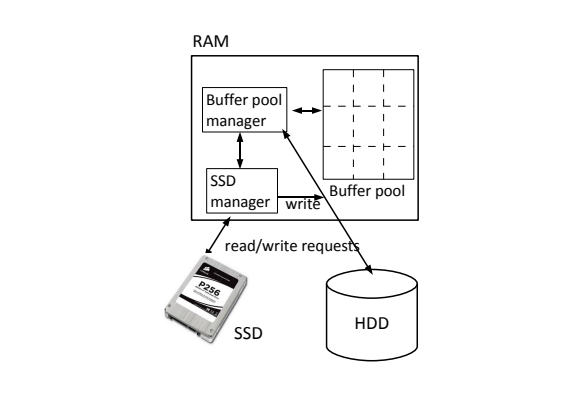
\includegraphics[width=0.5\textwidth]{hybrid.png}
    \caption{Hybrid Storage}
\end{figure}



We are interested in the use of hybrid storage systems, consisting of SSDs and HDDs, for database management. 
We present cost-aware replacement algorithms, which are aware of the difference in performance between SSDs and HDDs, for both the DBMS buffer pool and the SSDs.
In hybrid storage systems, the physical access pattern to the SSDs depends on the management of the DBMS buffer pool. 
We studied the impact of buffer pool caching policies on SSD access patterns.
Based on these studies, we designed a cost-adjusted caching algorithm to effectively manage the SSD: a two-level version of the GreedyDual algorithm which we have adapted for use in database systems. 

GreedyDual is actually a range of algorithms which gen  eralize well-known caching algorithms, such as LRU and FIFO. 
Initially, we present the GreedyDual generalization of LRU and our restriction to two retrieval costs.
GreedyDual associates a non-negative cost $H$ with each cached page $p$. 
When a page is brought into the cache or referenced in the cache, $H$ is set to the cost of retrieving the page into the cache. 
To make room for a new page, the page with the lowest $H$ in the cache, $H_{min}$, is evicted and the $H$ values of all remaining pages are reduced by $H_{min}$.
By reducing the H values and resetting them upon access, GreedyDual ages pages that have not been accessed for a long time. 
The algorithm thus integrates locality and cost concerns in a seamless fashion.
We refer to it as GD2L. \cite{10.14778/2536354.2536355}

Here is the GD2L algorithm for reading a page P:

\begin{minipage}[t]{0.8\textwidth}
    \begin{algorithm}[H]
        \KwIn{Page $P$, Cost $H$ for each page, 
        Cost $R_s$ of retrieving an SSD page and $R_d$ of retrieving an HHD page, 
        An inflation value $L$ representing for the future settings of $H$}
        \KwOut{Quene of pages placed on SSDs $Q_s$, Quene of pages placed on HDDs $Q_d$}
        \BlankLine
        \caption{GD2L Algorithm}
        \uIf{Page $P$ is cached}{
            compare LRU page of $Q_s$ with LRU page of $Q_d$\;
            evict the page $q$ that has the smaller $H$\;
            set $L = H(q)$\;
            bring $P$ into the cache\;
        }
        \uElseIf{Page $P$ is on the SSD}{
            $H(P) = L + R_s$\;
            put $P$ to the MRU of $Q_s$\;
        }
        \uElseIf{Page $P$ is on the HDD}{
            $H(P) = L + R_d$\;
            put $P$ to the MRU of $Q_d$\;
        }
    \end{algorithm}
    
\end{minipage}

\subsection{Query optimization}

Query optimization is a technique that allows the database system to optimize the execution of queries to improve performance.
The operating system can support query optimization by providing services such as query planning, query rewriting, and query execution.
These services can help reduce the latency of query execution and improve the performance of database systems.

In a query optimizer, there are three components, transformer, estimator and plan generator. 
The transformer takes parsed query as input which is represented by set of query blocks. 
It determines that if it is advantageous to change the form of the query to reduce the cost of execution.
The estimator determines the over all cost of execution plan. 
This estimator uses three different measures to determine cost which includes selectivity, cardinality and cost of execution.
And the plan generator explores various plans for query block by checking various access paths, join methods and join orders. 
After checking various paths, optimizer picks the path with the lowest cost.\cite{geeksforgeeks}
The architecture of the optimizer is shown as following Figure8.

\begin{figure}[h!]
    \centering
    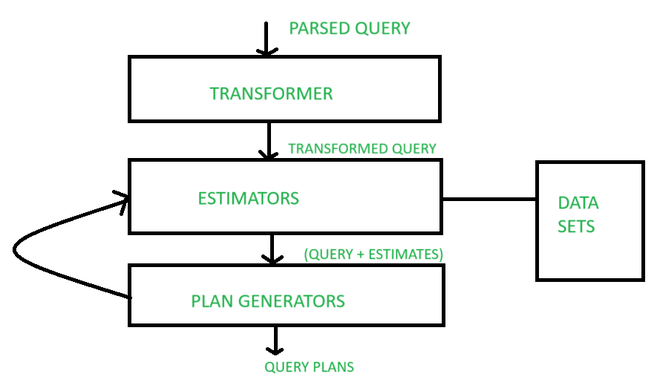
\includegraphics[width=0.7\textwidth]{query.png}
    \caption{Query Optimization}
\end{figure}

The query engine of a DBMS, transforms these queries into physical query execution plans. 
In this process, query optimization is the task of finding an optimal (or at least very good) physical execution plan with respect to the plan’s execution time.
It is crucial to find efficient query plans, because the execution times of different physical plans (that yield identical results) for the same query 
can vary by orders of magnitude and “the runtime system alone could never get that good performance without an optimizer”.\cite{Kossmann2022}

\subsection{Data Compression}

Data compression is a technique that allows the database system to reduce the size of data stored on disk.
The operating system can support data compression by providing services such as data compression algorithms, data decompression, and data storage.
These services can help reduce the storage space required for data and improve the performance of database systems by reducing the latency of disk I/O operations.

In order to reduce storage space and allow on-line query, how to trade off data compression effectiveness for on-line query performance is a challenge issue. 
We are concerned with an effective framework for temporal data set that does not scarify on-line query performance and is specifically designed for very large sensor network database. 
The sampled data are compressed using several candidate approaches including dictionary-base compress and lossless vector quantization. 
To take advantage of existing storage reduction mechanisms, 
the main idea of the developed framework is to encode raw data with a representation which requires less storage space. 
Hence, the data databases system can further apply their heuristics to prune the storage space.\cite{5641312}


\section{Summary}

In this report, we have discussed the operating system supports for database systems and how they can be optimized to improve performance and scalability.
We have focused on memory management, process scheduling, and file system management, and discussed how these aspects can be optimized to support database systems.


% References
\bibliographystyle{plain}
\bibliography{references} % Replace with your bibliography file

\end{document}